\documentclass[11pt]{article}
\setlength{\textheight}{210mm}
\setlength{\voffset}{4mm}
\setlength{\textwidth}{155mm}
\setlength{\oddsidemargin}{5mm}
\usepackage{graphicx, subfig}
\pagestyle{plain}
\begin{document}
\title{\vspace{-15ex}C++ Voting Model Implementation}
\author{Alexander Holiday\vspace{-2ex}}
\date{06/06/2013}
\maketitle
%% \begin{abstract}
%% The voting model detailed in \cite{durret:pnas12} is implemented in C++ in both rewiring regimes. The behavior of our implementation differs from that presented in \cite{durret:pnas12} for unknown reasons. In particular, while we observe the random walk behavior for certain values of alpha, the arc has support on (0, 1) regardless of the alpha under investigation. \cite{vazquez:prl08}.
%% \end{abstract}
\section*{Introduction}
The multi-opinion voting model detailed in \cite{durret:pnas12} was implemented in C++, including both rewire-to-same and rewire-to-random regimes. Results for two-opinion simulations over a range of $\alpha$ values and initial opinion distributions exhibit markedly different dynamics from those presented in \cite{durret:pnas12}. In particular, while we observe random walk behavior along arcs, these curves have support on (0,1) regardless of the $\alpha$ under investigation. Additionally, certain runs don't reach consensus in a number of steps on the same order of (or greater than) those suggested in \cite{durret:pnas12} this brief report reviews our simulation results and examines the possible sources of discrepancies.

\section*{Implementation}
The C++ code aims to replicate the model outlined in \cite{durret:pnas12}. Both rewire-to-same and rewire-to-random models are initialized as Erd\H{o}s R\'{e}nyi random graphs with average degree $\lambda$ (throughout this report $\lambda = 4$). To avoid $O(n^{2})$ intialization times, an algorithm based on geometrically distributed waiting times between edges in the adjacency matrix, detailed in \cite{?}, was used. The edges were also randomly assigned opinions (here, always either 0 or 1), based on some initial distribution $u_{0}=\{u_{1,0},u_{2,0}\}$. \\[1pt]
\indent During each step of a rewire-to-same simulation, an edge $e_{ij}$ is selected whose vertex ends $v_{i}$ and $v_{j}$ do not hold the same opinion (i.e. $\xi_{i}\neq\xi_{j}$ where $xi_{i}$ is the opinion of $v_{i}$). Then, with probability $\alpha$, the edge $e_{ij}$ is removed from the graph and reattached to a random vertex $v_{k}$ such that $\xi_{k}=\xi_{i}$ and $e_{ik}$ was not previously in the graph (the graph remains simple). Otherwise, with probability $1-\alpha$, we set $\xi_{i}=\xi_{j}$. This procedure is continued until the number of conflicts in the graph (the total number of edges $e_{ij}$ such that $\xi_{i}\neq\xi_{j}$) is zero. \\[1pt]
\indent The rewire-to-random model can differ from the one described above in one or two ways, each exhibiting significantly different dynamics. In the first variation, proposed in \cite{durret:pnas12}, the only change is that, during the rewiring stage, the new neighboring vertex of $v_{i}$ is chosen from the set of all other vertices, regardless of their opinion (while continuing to avoid parallel edges and loops). However, a small but significant second change is to allow the initial edge, $e_{ij}$, to be picked from any $e\in E(G)$ instead of dictating that $\xi_{i}\neq\xi_{j}$.  It was only with this second, additional adjustment that the model exhibited random walk behavior.
\section*{Results}

\begin{figure}[h!]
  \centering
  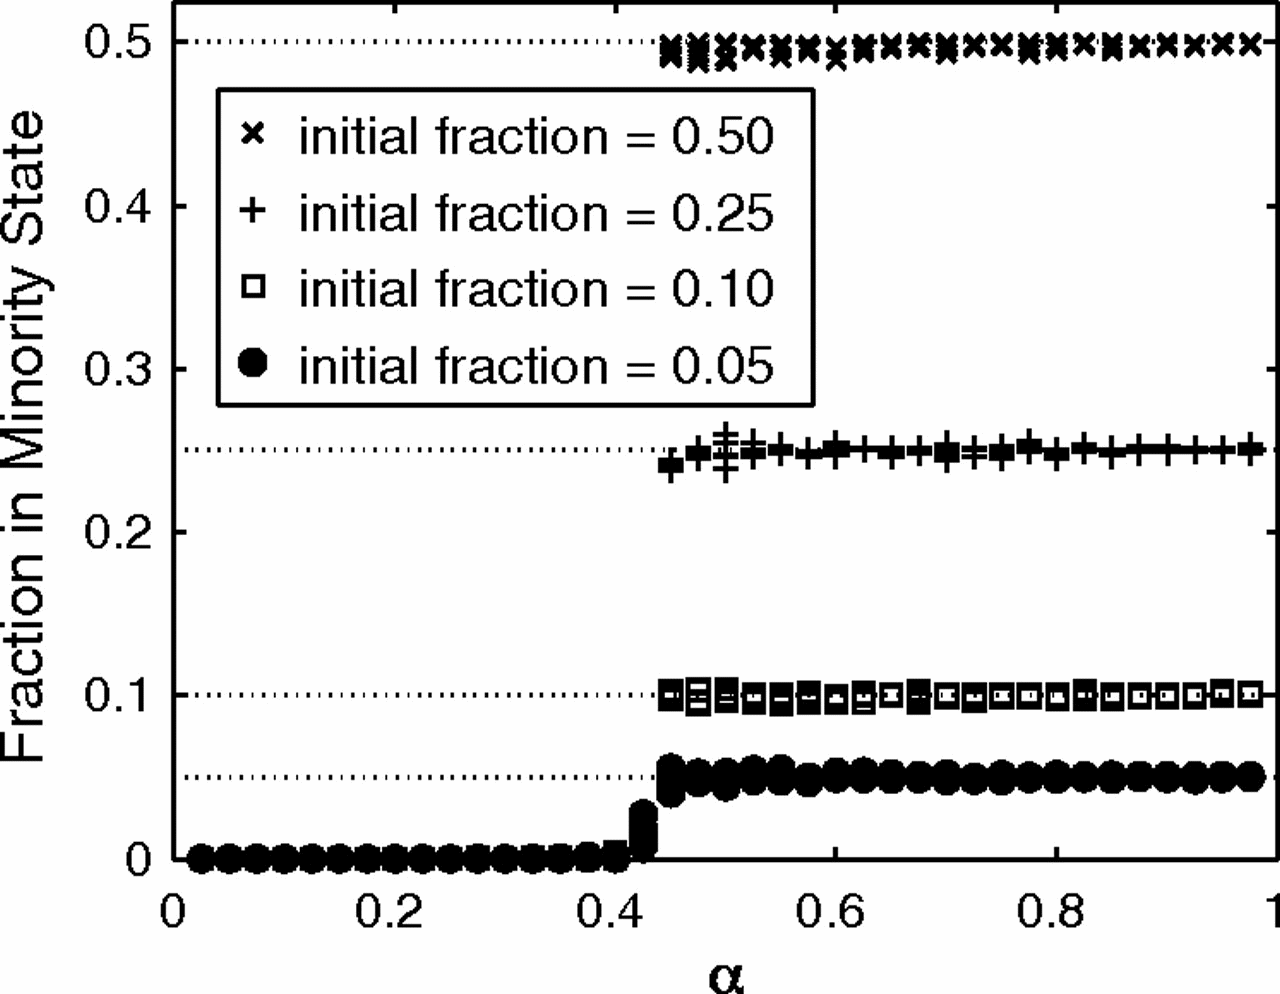
\includegraphics[height=55mm]{rwToSameBifDiag}
  \caption{Final minority fraction as a function of $\alpha$ and initial minority fraction (rewire-to-same), taken from \cite{durret:pnas12}.}
  \label{fig:durretRWtoSameBD}
\end{figure}

\begin{figure}[h!]
  \centering
  \subfloat[Only includes runs that have reached consensus]{
    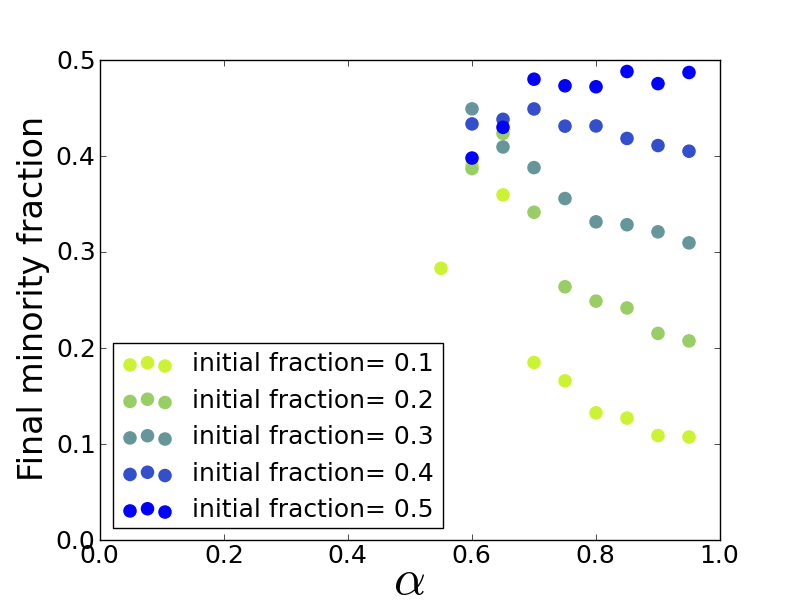
\includegraphics[width=65mm]{bifData_same_1000_4}
  }
  \hspace{3mm}
  \subfloat[Includes all runs, even if conflicts exist at the simulation's end] {
    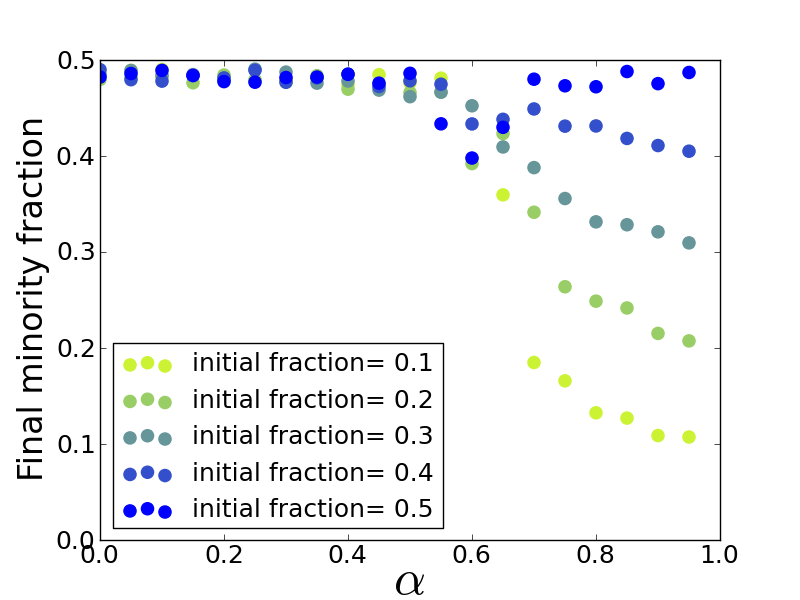
\includegraphics[width=65mm]{bifData_noConvergence_same_1000_4}
  }
  \caption{Same data as Fig. \ref{fig:durretRWtoSameBD}, taken from our implementation}
  \label{fig:myRWtoSameBD}
\end{figure}

\begin{figure}[h!]
  \centering
  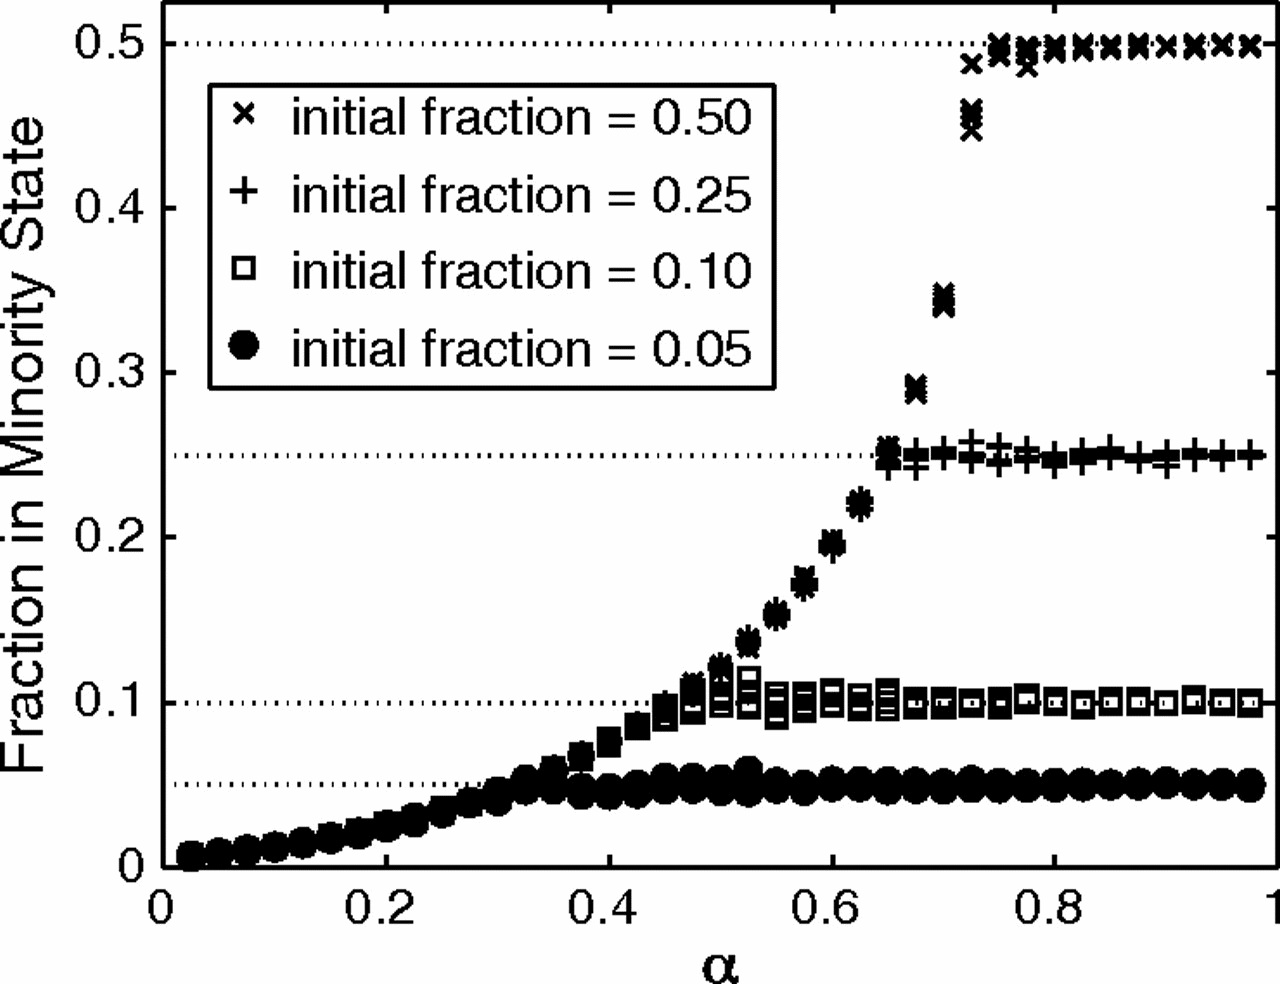
\includegraphics[height=55mm]{rwToRandomBifDiag}
  \caption{Final minority fraction as a function of $\alpha$ and initial minority fraction (rewire-to-random), taken from \cite{durret:pnas12}.}
  \label{fig:durretRWtoRandomBD}
\end{figure}


\begin{figure}[h!]
  \centering
  \subfloat[Runs that reached consensus]{
    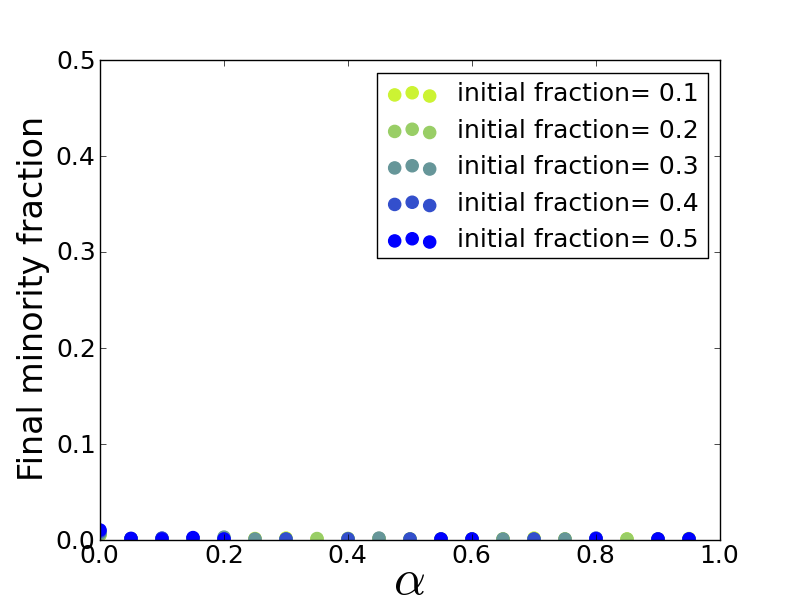
\includegraphics[width=65mm]{bifData_randomIeqJ_1000_4}
  }
  \hspace{3mm}
  \subfloat[All runs] {
    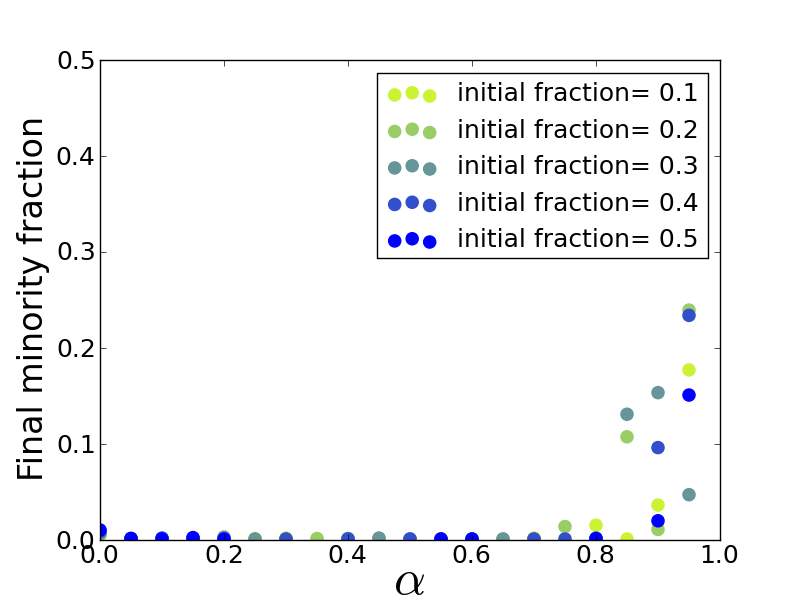
\includegraphics[width=65mm]{bifData_noConvergence_randomIeqJ_1000_4}
  }
  \caption{Data corresponding to Fig. \ref{fig:durretRWtoRandomBD} from our implementation. In these simulations edges $e_{ij}$ were chosen so that $\xi_{i}=\xi_{j}$.}
  \label{fig:myRWtoRandomBD}
\end{figure}

\begin{figure}[h!]
  \centering
  \subfloat[Runs that reached consensus]{
    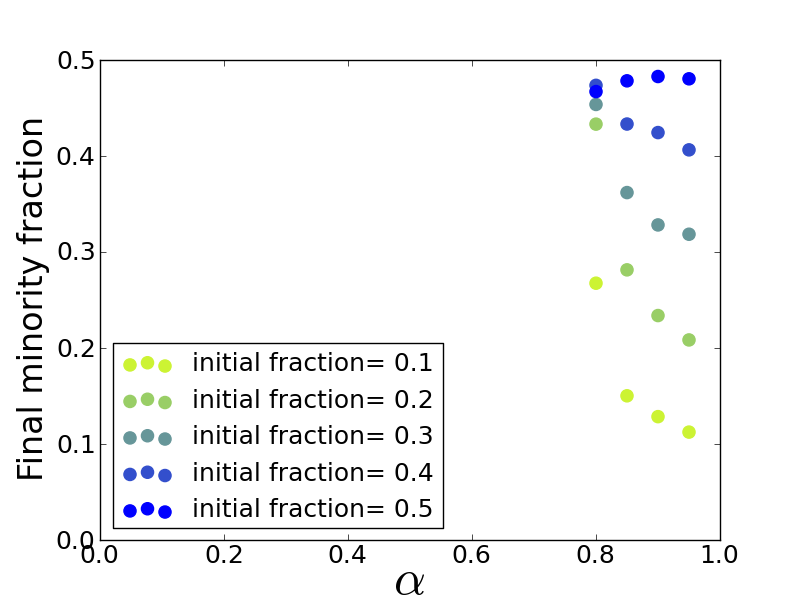
\includegraphics[width=65mm]{bifData_randomIneqJ_1000_4}
  }
  \hspace{3mm}
  \subfloat[All runs] {
    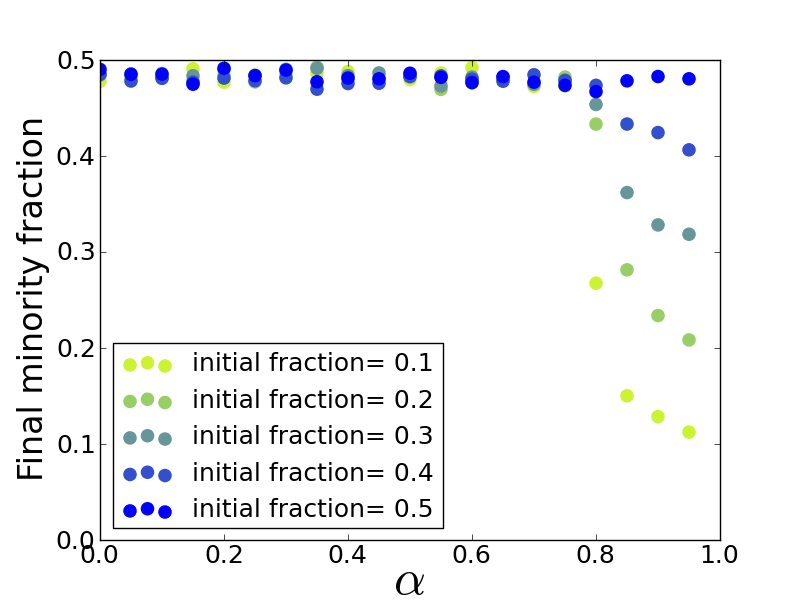
\includegraphics[width=65mm]{bifData_noConvergence_randomIneqJ_1000_4}
  }
  \caption{Data corresponding to Fig. \ref{fig:durretRWtoRandomBD} from our implementation. In these simulations edges $e_{ij}$ were chosen from $V(G)$.}
  \label{fig:myRWtoRandomBD}
\end{figure}

\begin{figure}[h!]
  \centering
  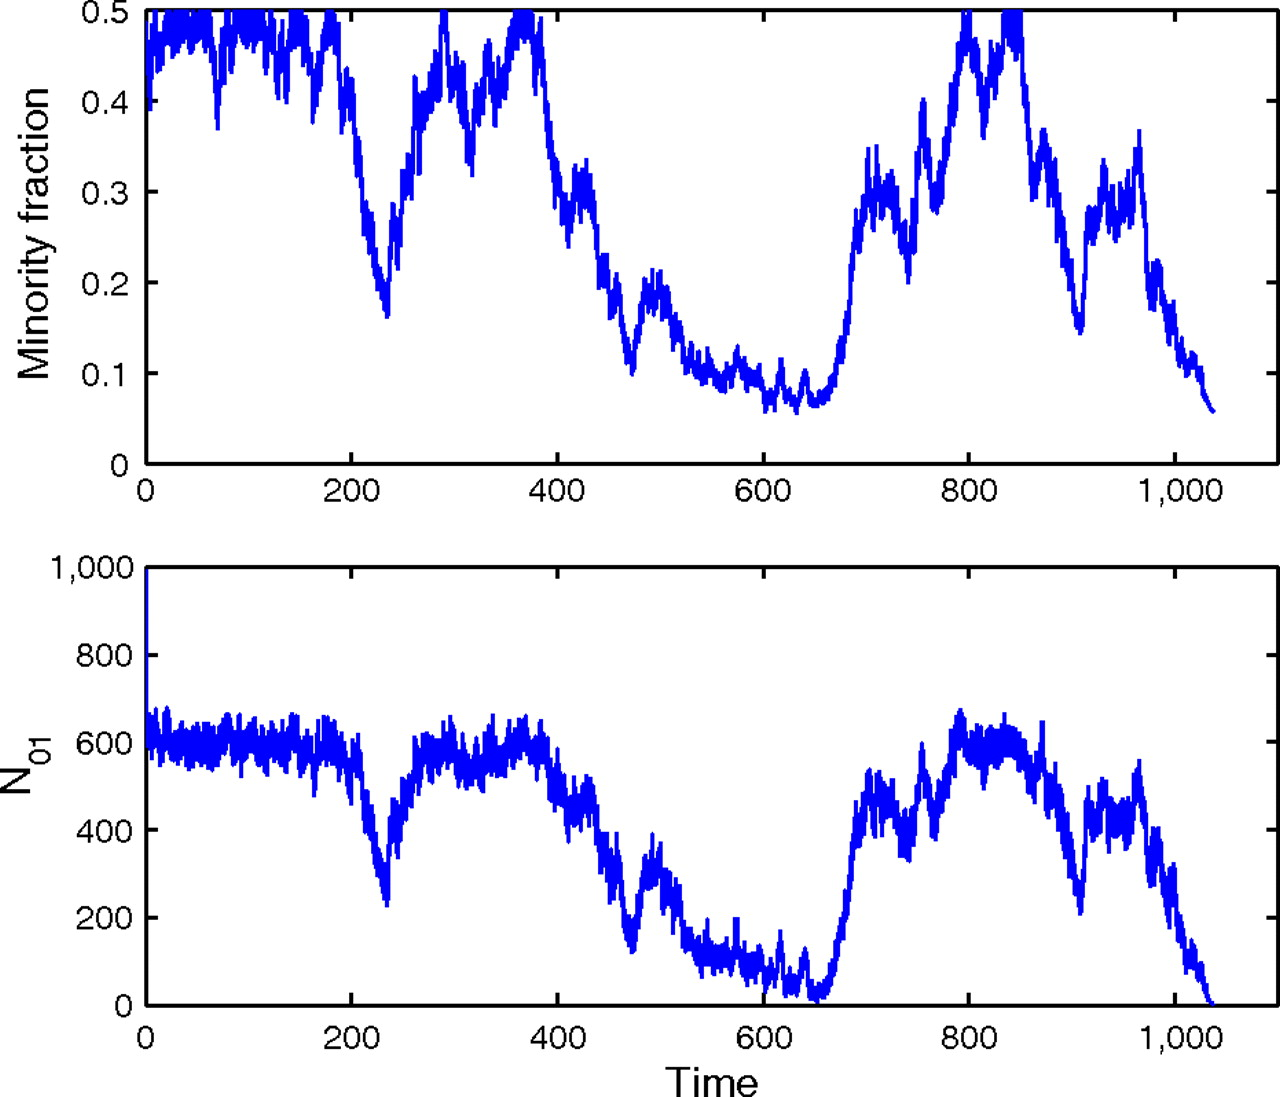
\includegraphics[height=55mm]{durretTimeCourses}
  \caption{Evolution of conflicting edges and minority fraction, taken from \cite{durret:pnas12}.}
  \label{fig:durretTimeCourses}
\end{figure}

\begin{figure}[h!]
  \centering
  \subfloat[Runs that failed to reach consensus, $\alpha=0.5$.]{
    \includegraphics[width=65mm]{{graphStats_randomIneqJ_1000_4_0.5_0.5_0.5_noConsensus}.png}
  }
  \hspace{3mm}
  \subfloat[Run that reached consensus, $\alpha=0.8$.] {
    \includegraphics[width=65mm]{{graphStats_randomIneqJ_1000_4_0.8_0.5_0.5_consensus}.png}
  }
  \caption{Evolution of conflicting edges in rewire-to-same from same.}
  \label{fig:myIneqJTCs}
\end{figure}

\begin{figure}[h!]
  \centering
  \includegraphics[width=65mm]{{graphStats_randomIeqJ_1000_4_0.5_0.5_0.5_consensus}.png}
  \caption{Evolution of conflicting edges in rewire-to-same from all.}
  \label{fig:myIeqJTC}
\end{figure}

\begin{figure}[h!]
  \centering
  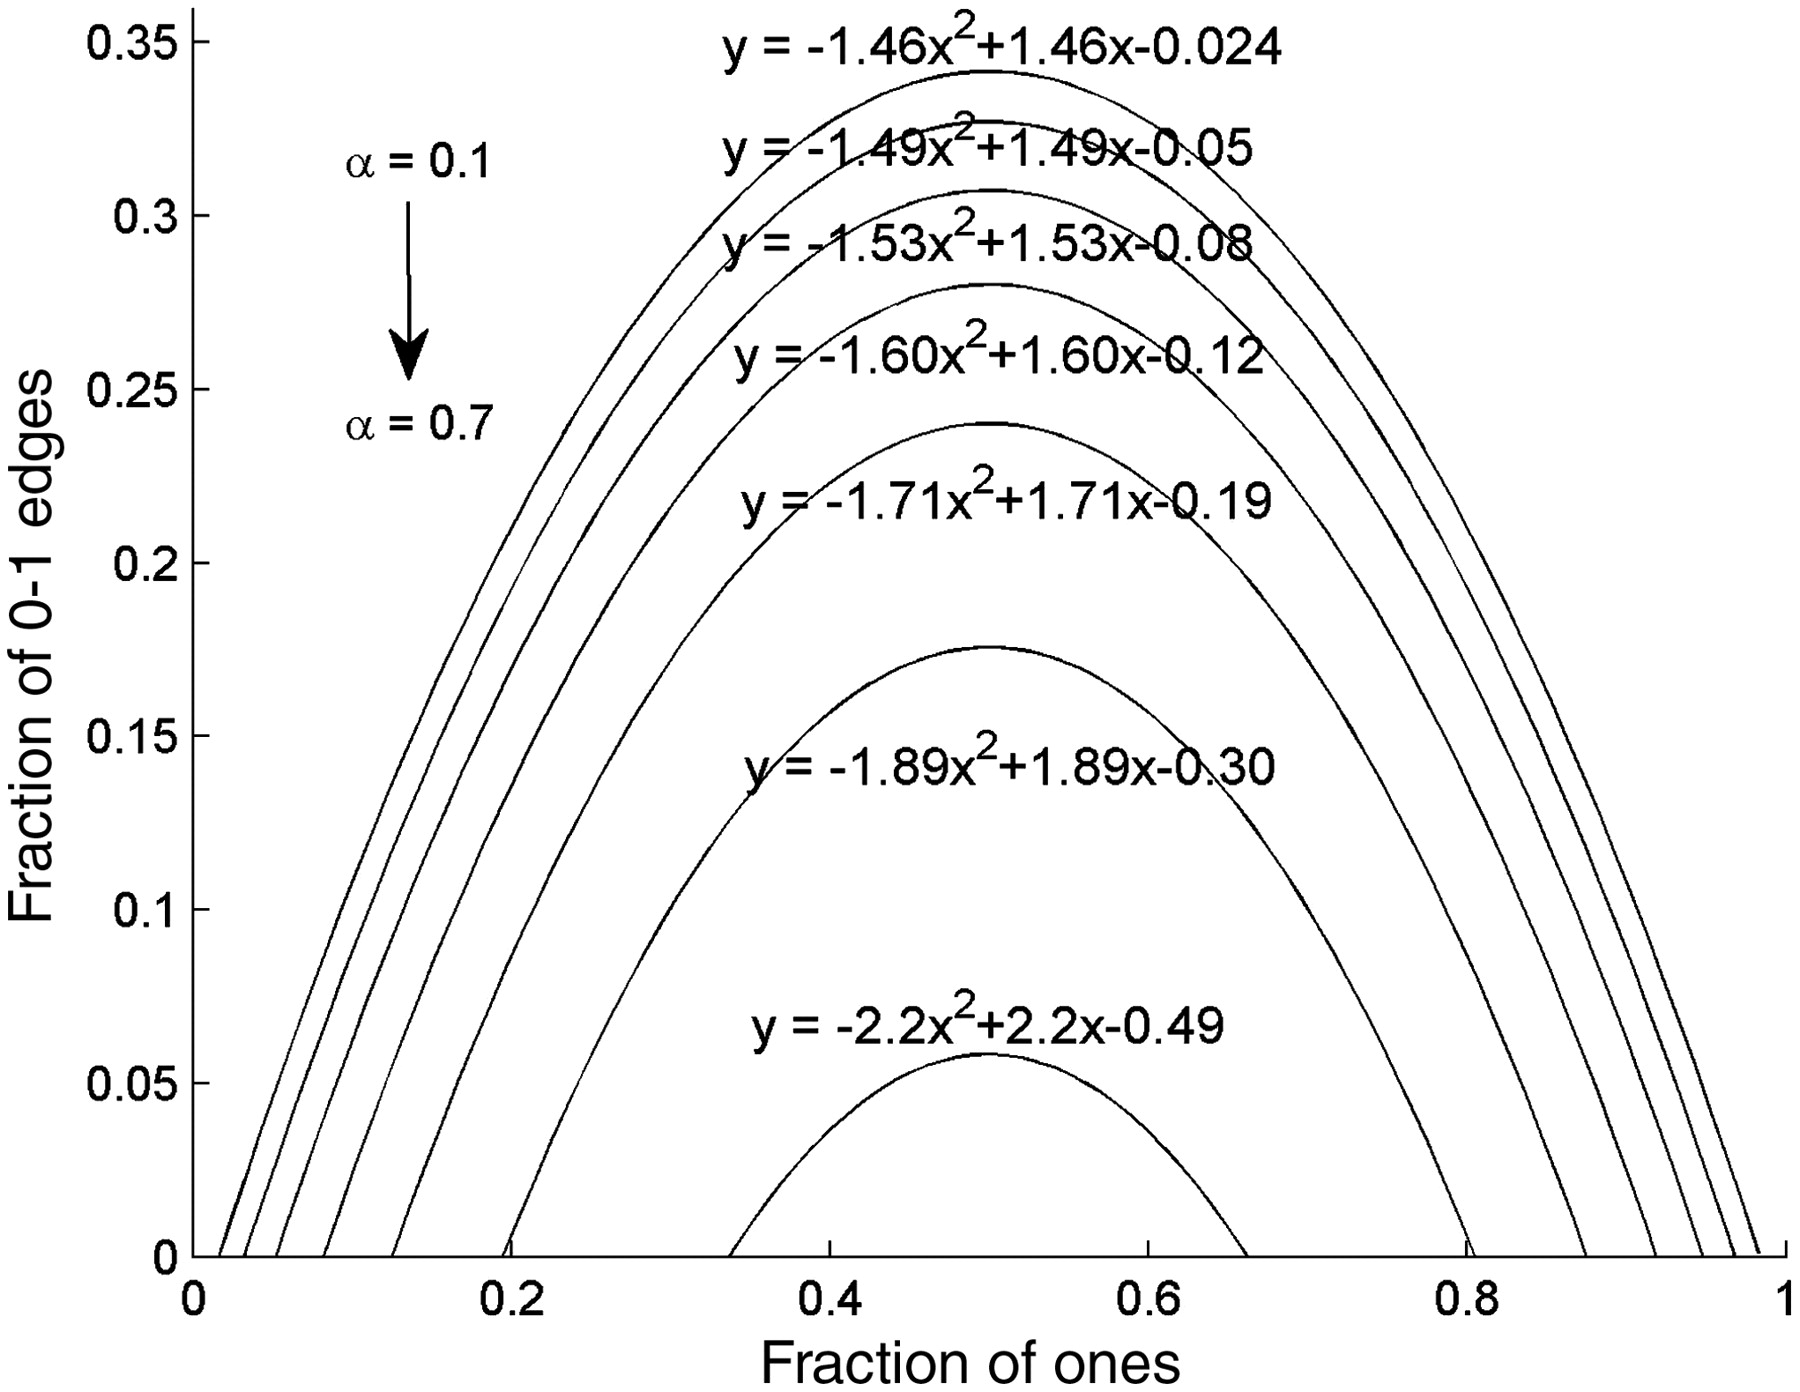
\includegraphics[height=55mm]{durretArcs}
  \caption{Random walk arcs as a function of $\alpha$, from \cite{durret:pnas12}}
  \label{fig:durretArcs}
\end{figure}

\begin{figure}[h!]
  \centering
  \subfloat[$e_{ij}\in \{e \in E(G) \mid \xi_{i} \neq \xi_{j}\}$]{
    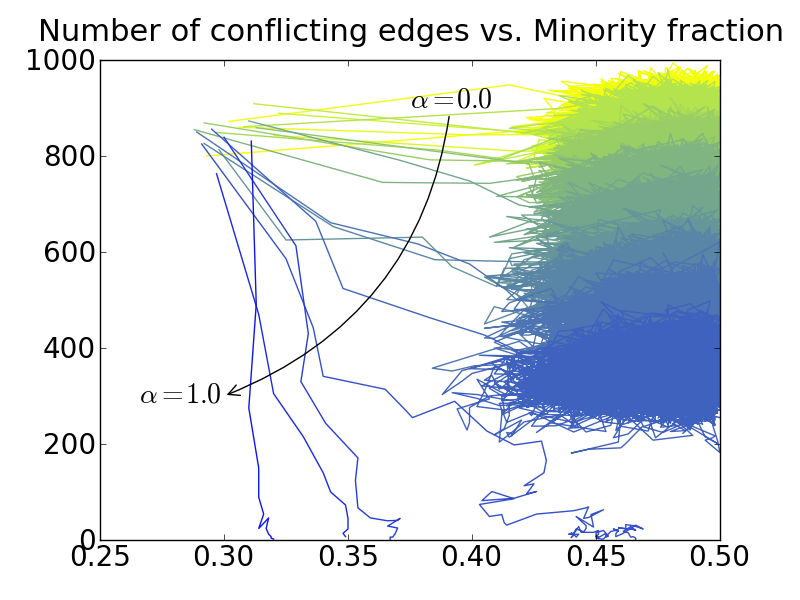
\includegraphics[width=65mm]{nData_randomIneqJ}
  }
  \hspace{3mm}
  \subfloat[$e_{ij}\in E(G)$] {
    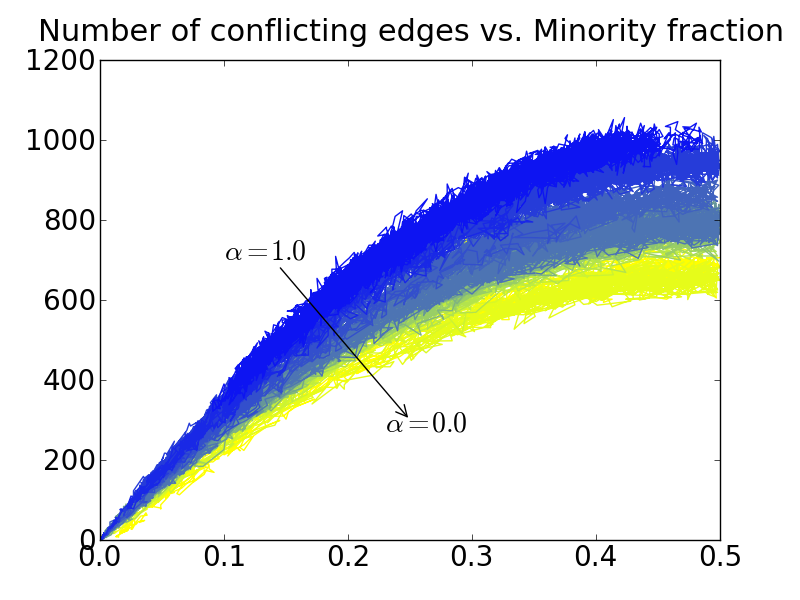
\includegraphics[width=65mm]{nData_randomIeqJ}
  }
  \caption{Random walk arcs from the two different implementations.}
  \label{fig:myArcs}
\end{figure}

\section*{Future work}
future work

\bibliographystyle{abbrv}
\bibliography{votingBib}
\end{document}
